\documentclass{ltjsbook}
\usepackage{docmute} 
\usepackage{myStyle} 

\begin{document}
\chapter{Rによる帰無仮説検定}
\label{chapter20} 


\label{chapter20}
ここまで様々な統計的仮説検定を学んできましたが，実践上はどのように行うのかを知らなければ絵に描いた餅になります。今回は統計環境Rで帰無仮説検定を行う方法について，実際に手を動かして理解を深めてください。統計環境はRを，その補助としてRStudioを用います。
統計パッケージは以外にも色々ありますが，どのようなパッケージ，ソフトを使っても同様の出力が得られます。大事なことは，出力画面の位置で内容を覚えるのではなく，意味的な理解をしておくことです。

\section{基本的操作のおさらい；記述統計}
\subsection{環境の確認}
まずはRとRStudioの使い方を再確認してください。RStudioはRを使うための統合環境です。
\paragraph{RStudioの起動}RStudioを起動してください。パッケージのインストールをするときなど，管理人権限が必要になるケースがあります。
\paragraph{プロジェクトを開く}RStudioは「プロジェクト」としてファイルや実行環境を管理できます。プロジェクトは1つのフォルダ(ディレクトリ)を作成しますから，その中にスクリプトファイル(.Rファイル)を保存すると良いでしょう。この授業用，あるいは今回のセクション用にプロジェクトを新規作成してください\footnote{第\ref{chapter4}講で使ったプロジェクトを再利用しても構いません。}。プロジェクトを新規作成，あるいは開くことができたら，RStudioの右上などで，プロジェクトが開いていることを確認しましょう($\to$図\ref{fig::20_01})。
\begin{figure}[ht]
    \centering
    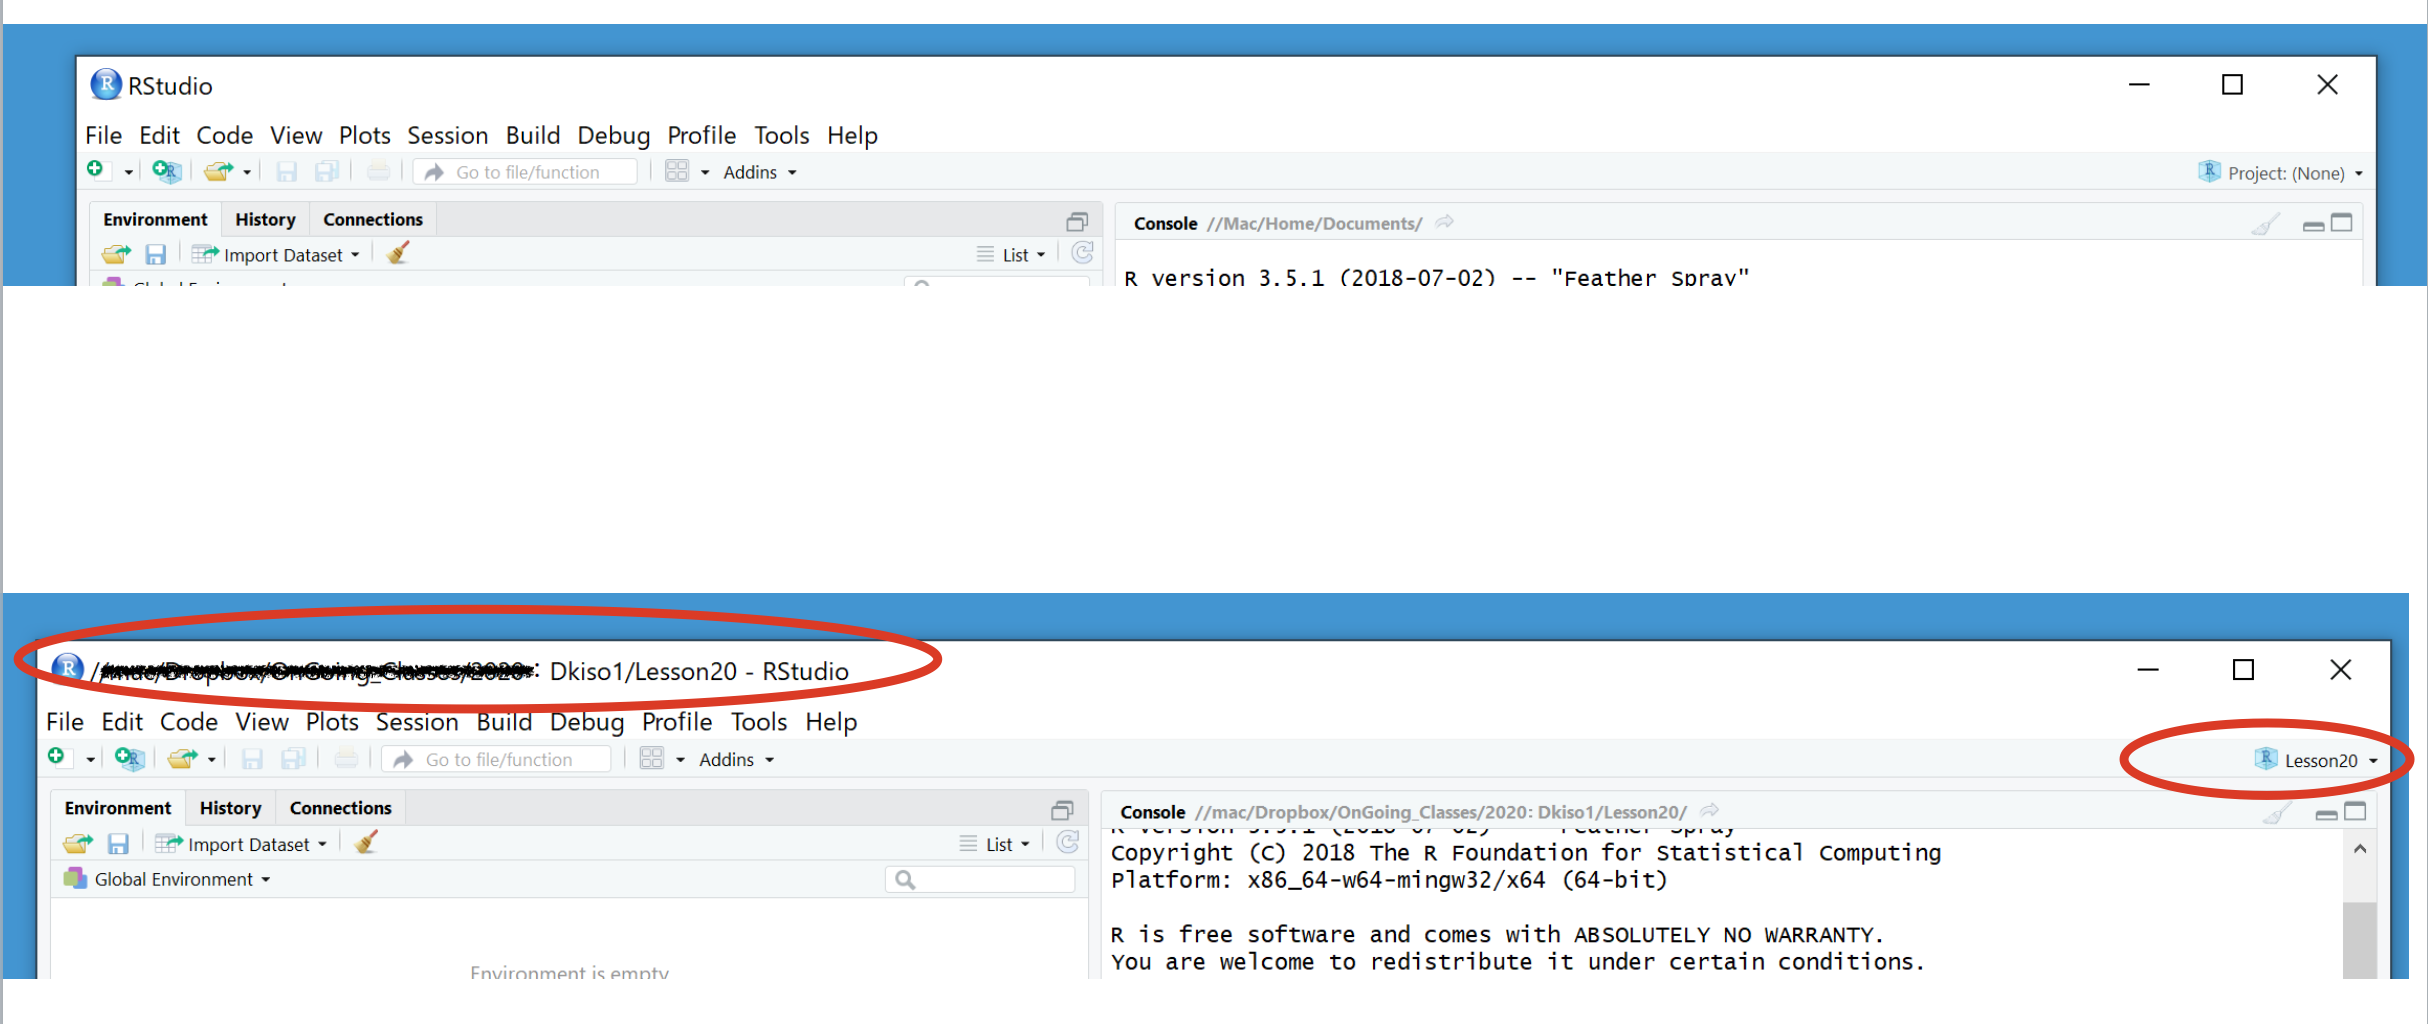
\includegraphics[keepaspectratio,width=12cm]{images/text20/fig20_01.png}
    \caption{プロジェクトが開いていることを確認する。上が開いていない状態。下が開いている状態。開いていると，メニューバーにフォルダが表示され，右上にプロジェクト名が表示されている。}
    \label{fig::20_01}
\end{figure}

\paragraph{Rスクリプトを開く}今日のコードを書くためのRスクリプトファイルを準備します。\verb|File > NewFile > R Script|と進み，何も書いてないRスクリプトの画面を表示させてください。真っ白いファイルが開いたら準備完了です。

\subsection{データセットを作る}
\paragraph{データに変数を代入}
第\ref{chapter16}講でやったように，小さなサイズの母集団を作ってそこから標本をいくつも取り出す練習をしてみましょう。\texttt{code:\ref{code::20_01}}を入力してください\footnote{\#はコメントアウトで「この行で何を計算しているか」を説明している箇所です。みなさんが必ずしも入力する必要はありません。ただ，コメントアウトをつけておくと後で読み返しやすくなります。}。

\begin{lstlisting}[language=c++,label={code::20_01},caption={繰り返しサンプリングする}]
# Clear workspace
rm(list=ls())
### 母集団を作る
X <- rnorm(100,5,1)
## 母平均
mean(X)
### 標本1を作る
s1 <- sample(X,5)
## 標本平均
mean(s1)
## 以下繰り返し
s2 <- sample(X,5)
mean(s2)
s3 <- sample(X,5)
mean(s3)
s4 <- sample(X,5)
mean(s4)
s5 <- sample(X,6)
mean(s5)
\end{lstlisting}

Rでの確率関数は，関数の名前の前に\texttt{r}をつければ乱数を発生させる，というのがありましたね($\to$第\ref{chapter7}講)。
正規分布は\verb|normal distribution|で，Rの中では\texttt{normal}という関数を使いますから，正規\underline{乱数}は\texttt{rnorm}と書くのでした。また，正規分布は平均と標準偏差によって位置や幅が変わりますから，これを引数\footnote{引数は「ひきすう」と読みます。関数に与える数字やオプションの指定などのことを総称してこのように呼びます。}にとって\texttt{rnorm(N, mean, sd)}とすることで，平均と標準偏差を指定した乱数を$N$個作ることができるのでした(ここでは一般化するためにこのように書いていますが，実際は$N,mean,sd$のところには入れたい数字が入ります。平均50,標準偏差10の乱数を100個つくるのであれば，\texttt{rnorm(100,50,10)}のように\footnote{引数を明示的に指定することもできます。\texttt{rnorm(n=100,mean=50,sd=10)}のようにです。このようにする場合は，引数の順序に制限がなくなりますから，\texttt{rnorm(mean=50,n=100,sd=10})のように書いても構いません。逆に明示しない場合は，前から順に個数，平均，標準偏差だ，と解釈されます。})

さてここのコードですが，4行目の\texttt{rnorm}関数で平均5，標準偏差1の乱数を100個作りました。これを母集団と考えます。オブジェクト$X$に代入するため，\verb|<-|（「小なり」と「ハイフン」)で矢印記号を作っています。これが母集団ですから，母平均は\texttt{mean(X)}で計算できます。

次に\texttt{sample}関数で，変数名\texttt{X}として作った母集団から5個のサンプルを無作為に抜き出してオブジェクトに代入しています(8行目など)。サンプルの平均はまた，それぞれのオブジェクトを\texttt{mean}関数で計算できます。

標本平均が母平均の推定値として，どれほど適切なのかをチェックしてみてください。また標本平均の平均のほうが，より母平均に近くなっている・・・でしょうか？\footnote{データを乱数で作っているので，実現値次第では必ずしもそうならないことがあります。その場合は何度か試してみるか，母集団・標本のサイズを大きくして検証してください。実際に100人分のデータを集めたり，何度もサンプリングを繰り返すのは大変ですが，機械の中でやることですので簡単に状況設定を弄ることができます。}

続いて標準偏差を計算してみましょう\footnote{これ以降，s1のサンプルは個々人の実行環境によって違うと思いますので，アウトプットは示していません。}(\texttt{code:\ref{code::20_01}})。標準偏差の関数は\texttt{sd}です。また，分散は\texttt{var}で得られます。
\begin{lstlisting}[language=c++,label={code::20_02},caption={関数で標準偏差や分散を求める}]
# 標準偏差
sd(s1)
# 分散
var(s1)
# 標準偏差 の二乗は分散に等しい
sd(s1)^2
\end{lstlisting}
標準偏差は分散の正の平方根ですから，統計量として持っている意味は同じです。確認のために最後の1つの式を入れました。6行目で\texttt{\^}とあるのは累乗の計算記号です。

ところで注意してもらいたいのですが，Rがデフォルトで持っている標準偏差(と分散)の関数は，不偏分散に基づいています。つまり，足したデータの総数ではなく，総数$-1$で割ったものになっています。標本分散，標本標準偏差が欲しい時は，計算式を書いて計算しなければなりません。\texttt{code:\ref{code::20_03}}を書いて確認してみましょう。
\begin{lstlisting}[language=c++,label={code::20_03},caption={標本分散を求める}]
# 標本分散
mean((s1 - mean(s1))^2)
# 確認
var(s1)*4/5
\end{lstlisting}

標本分散の式(2行目)は，複数の式が入れ子になっています。まず\texttt{s1 - mean(s1)}でデータセット$s1$から平均を引いています。平均値は1つ，$s1$は5つの要素がなるベクトルですが，このような場合Rは平均を自動的に使い回し，$s1$の各要素から平均値を引き算するようにしています。つまり，平均偏差ベクトルがここで作られています。それを\texttt{\^　2}で二乗し，総和して総数で割る=\texttt{mean}関数を使う，という計算です。

確認のところは，不偏分散が$N-1=4$で割っているものですから，4倍して$N=5$で割り直す，という計算をしています。

\subsection{確率分布関数の利用}
次に第\ref{chapter17}講での例を使って，確率関数の計算をしてみましょう。Rによる確率変数の呼び出し方の違いをもう一度確認しておいてください(図\ref{fig::20_02})。
\begin{figure}[ht]
    \centering
    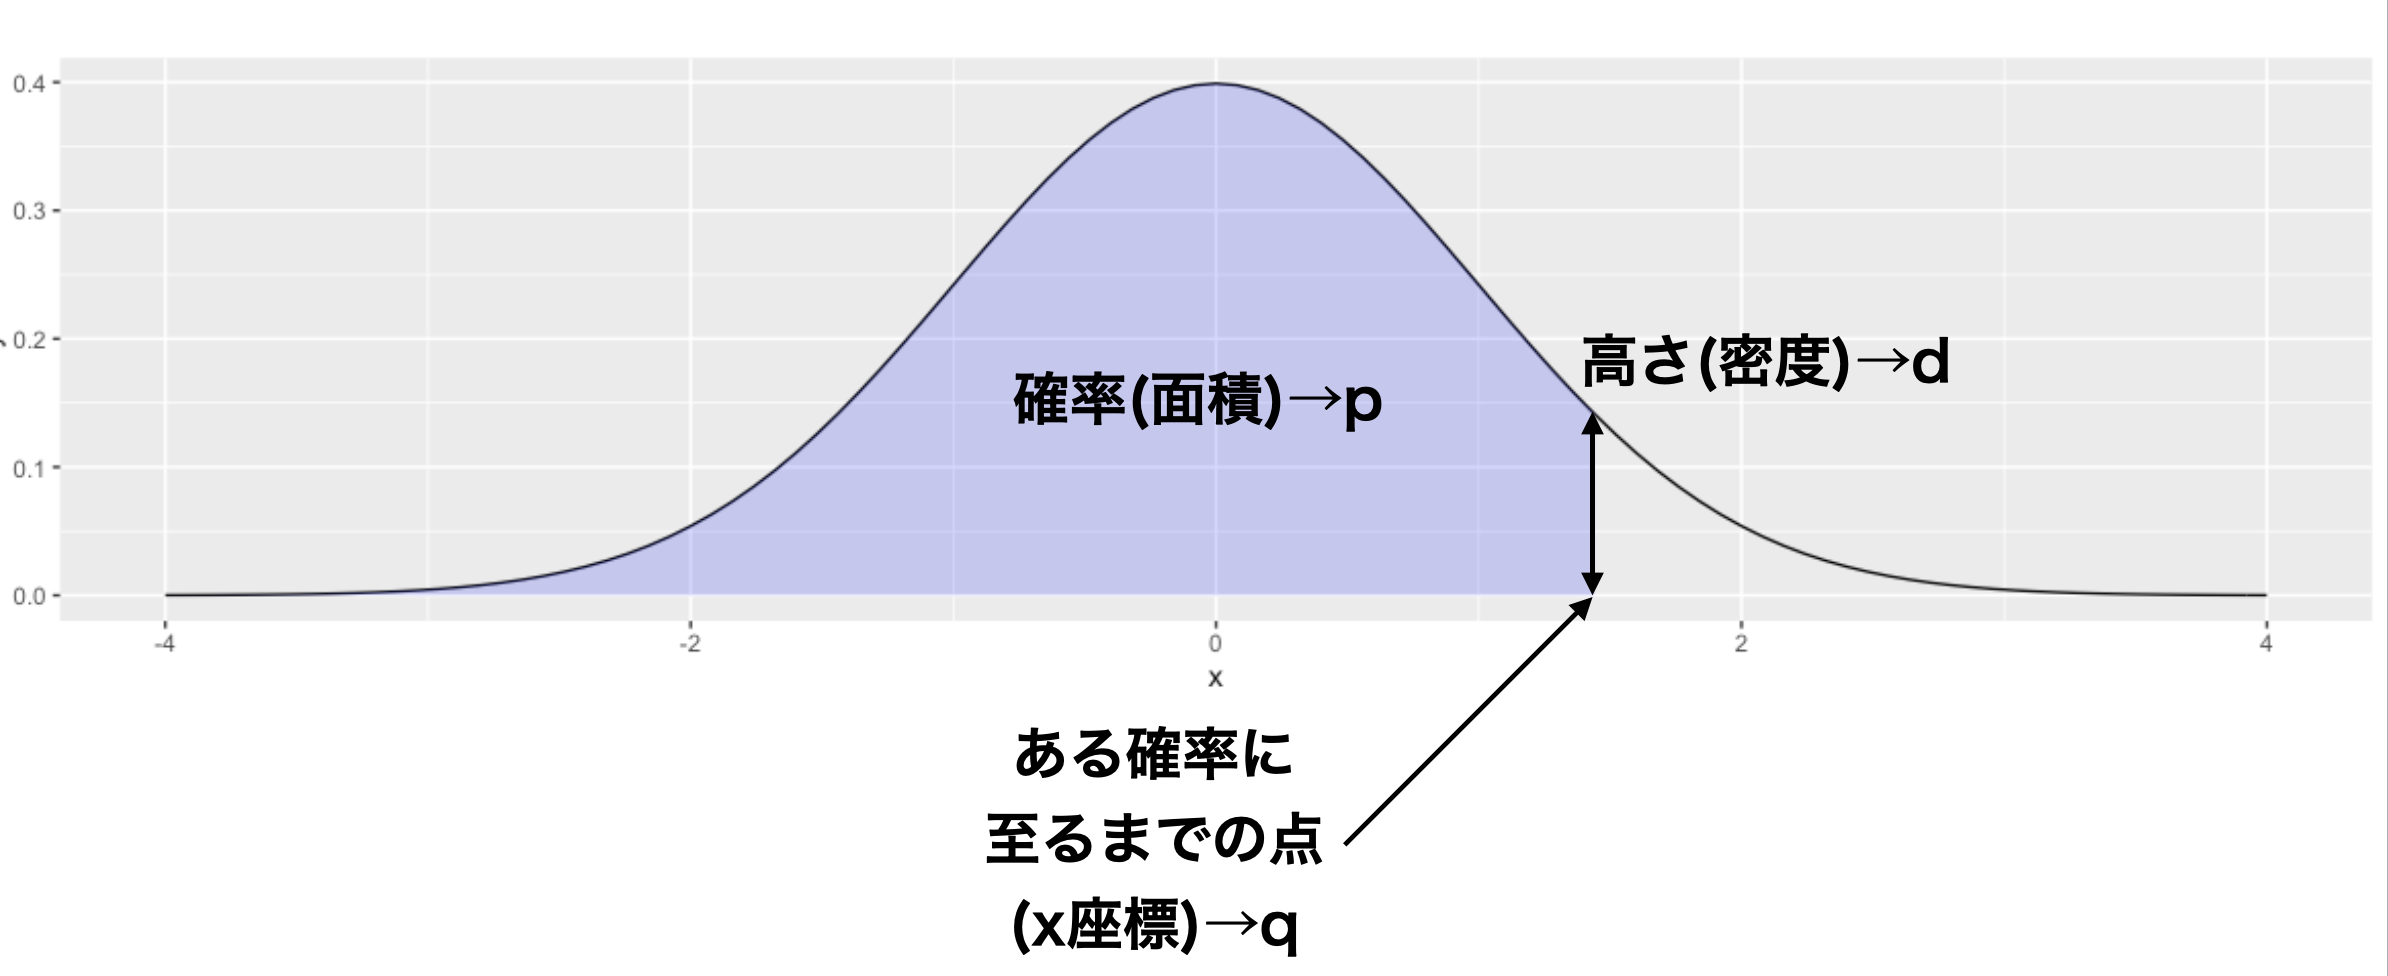
\includegraphics[keepaspectratio,width=12cm]{images/text20/fig20_02.png}
    \caption{\texttt{dnorm,pnorm,qnorm}の違い}
    \label{fig::20_02}
\end{figure}

これを踏まえて，まずは95\%信頼区間で区間推定するところです。ピークを挟んで95\%の面積が欲しいのですから，
\begin{enumerate}
    \item ピークを挟んで95\%の幅が欲しい
    \item 確率の総面積は1なので，両端に5\%残したいことになる
    \item ということは、片側に2.5\%あれば良い
    \item x座標が欲しいので，したから97.5\%の確率点を\texttt{qnorm}で求める
\end{enumerate}
という手順になるのでした(図\ref{fig::20_03})。コードでは\texttt{code:\ref{code::20_04}}のようにすればOKです。
\begin{figure}[ht]
    \centering
    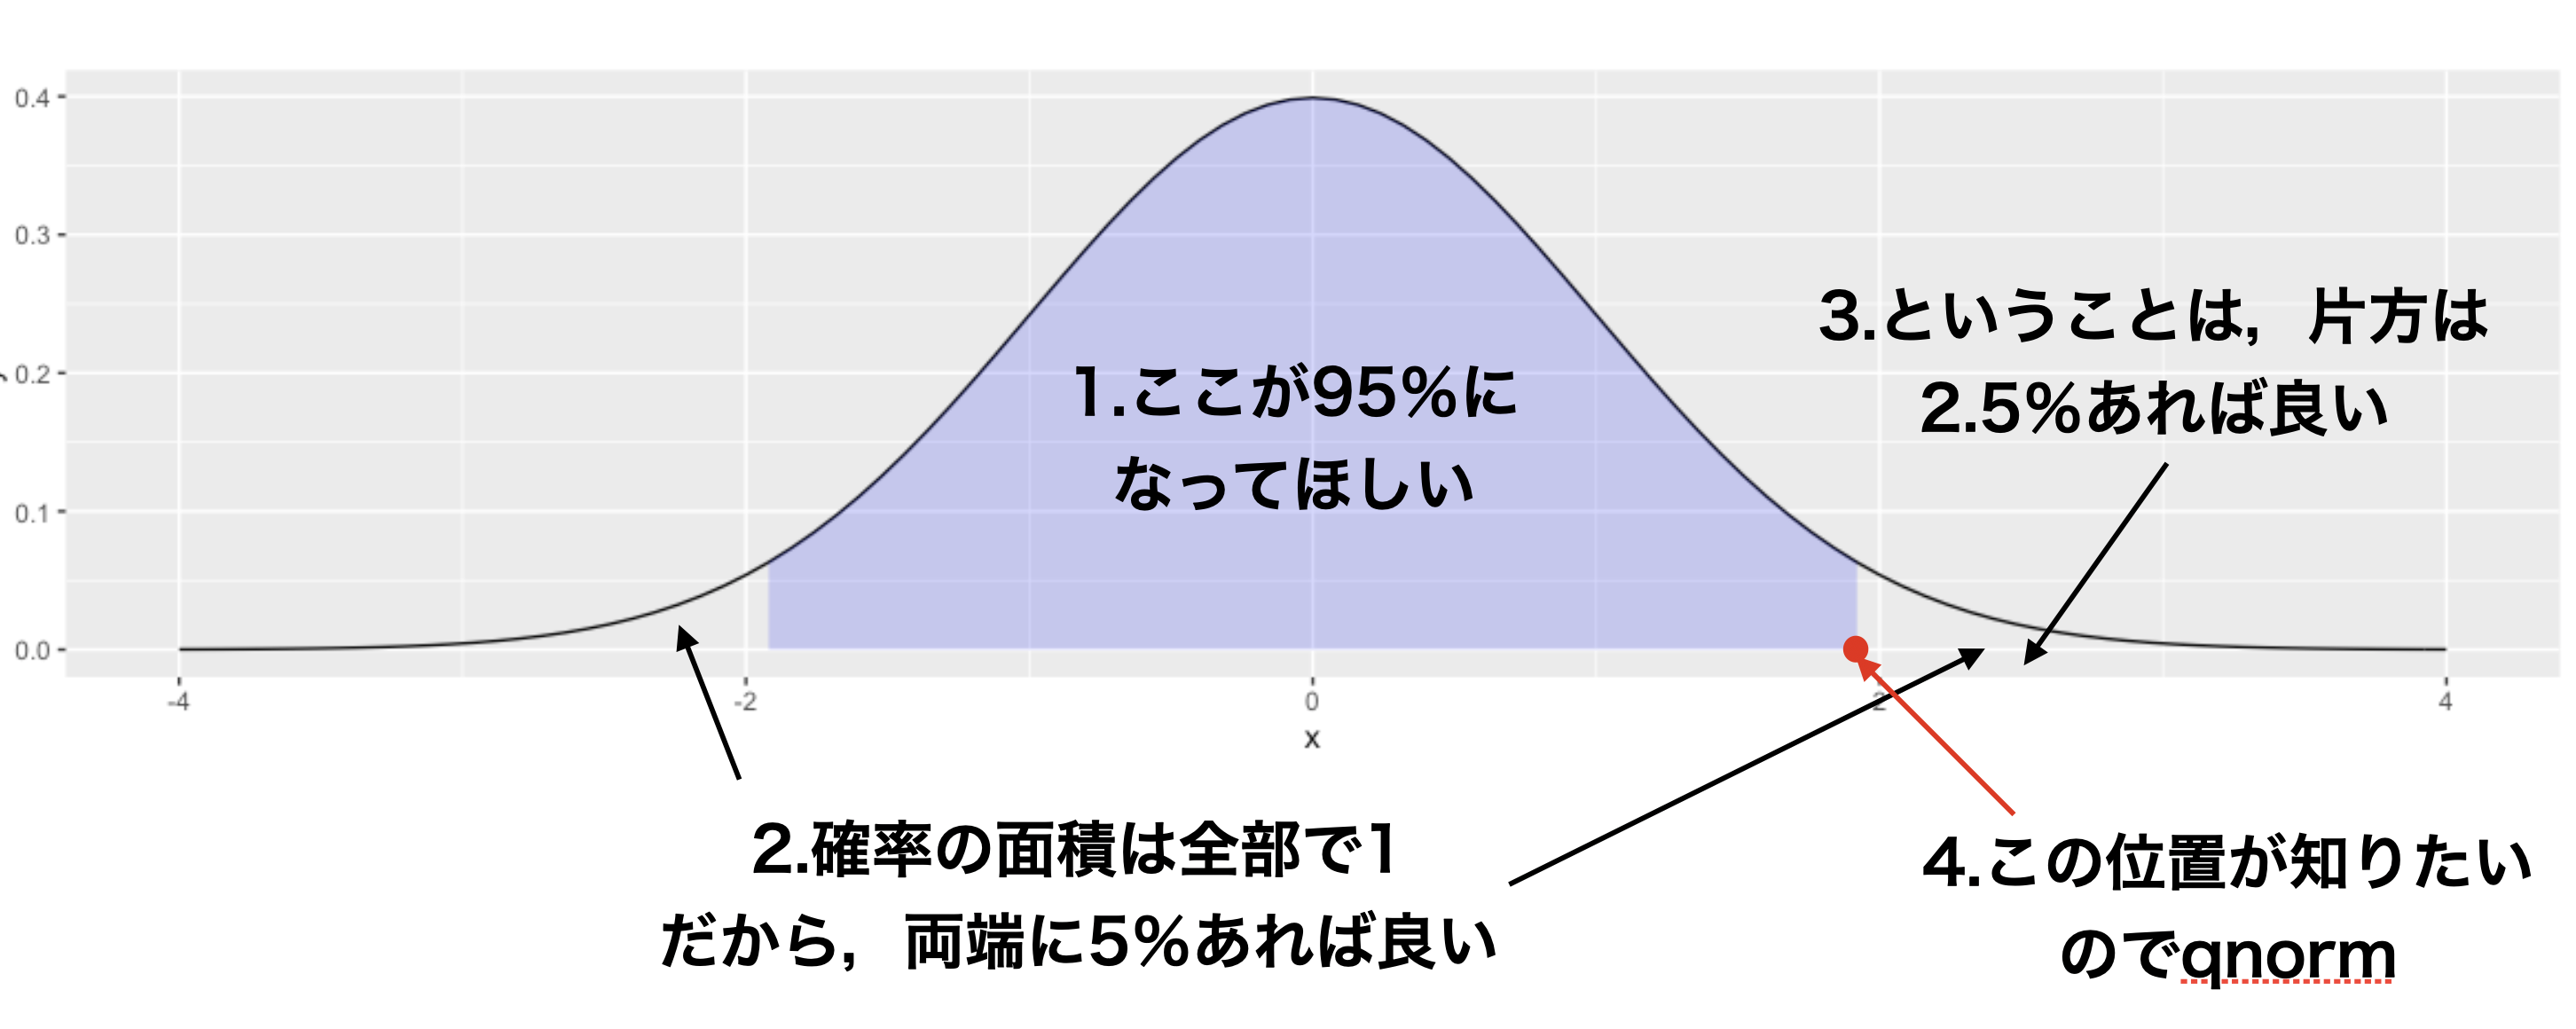
\includegraphics[keepaspectratio,width=12cm]{images/text20/fig20_03.png}
    \caption{95\%の確率点を求めるロジック}
    \label{fig::20_03}
\end{figure}

\begin{lstlisting}[language=c++,label={code::20_04},caption={正規分布の95\%区間}]
# 正規分布の95%区間
qnorm(0.975, mean = 0, sd = 1)
\end{lstlisting}
これで区間推定してみましょう。今回は母平均5,母標準偏差1のところからサンプルをとってきています。例えば1つ目のオブジェクト，$s1$について区間推定するならば，\texttt{code:\ref{code::20_05}}として計算できることになります\footnote{-1.96のところを，下から0.025の確率点で算出することでマイナス符号をつけないで表現できています。}。
\begin{lstlisting}[language=c++,label={code::20_05},caption={標本1の区間推定}]
    mean(s1)+qnorm(0.025)*(1/sqrt(5))
    mean(s1)+qnorm(0.975)*(1/sqrt(5))
\end{lstlisting}


ただし，これは母分散がわかっている場合であって，実際はわからないので$t$分布を使うのでした。Rにおける$t$分布の関数名はそのまま\texttt{t}なので，これを\texttt{dt,pt,qt}などとすれば確率密度や累積確率，確率点がわかります。ただし，引数として自由度$df$が必要なことを忘れないで。これを使った区間推定は，\texttt{code:\ref{code::20_06}}のようになります\footnote{自由度の設定と，母分散の変わりに標本分散\texttt{sd(s1)}とすることに注意。}。
\begin{lstlisting}[language=c++,label={code::20_06},caption={母分散がわからない場合}]
    mean(s1)+qt(0.025,df=4)*(sd(s1)/sqrt(5))
    mean(s1)+qt(0.975,df=4)*(sd(s1)/sqrt(5))
\end{lstlisting}
それにしても，数式を書くので何やら思ったより面倒だな，と思った人もいるかもしれません。実はもっと簡単な方法があります。それは，Rの$t$検定の関数を使う方法です。$t$検定といえば，2群の平均値差についての検定が思いつきますが，それは次のセクションでやることにして，\texttt{code:\ref{code::20_07}}を実行してください。
\begin{lstlisting}[language=c++,label={code::20_07},caption={t.test関数で推定}]
    t.test(s1,mu=5,conf.level = 0.95)
\end{lstlisting}
これは，母平均が5である母集団から得られた標本の平均が，母集団から有意に離れているかどうかを検定するという検定方法になります。これを実行すると，私の環境では\texttt{console\ref{RS:out20_01}}のような結果が得られました\footnote{繰り返しになりますがs1のサンプルは実行環境によって違うと思いますので，結果はみなさんの手元の数字と異なると思います。出力のどこがどういう意味であるかを見ることが肝要です。}。

\begin{Rscreen}{t.testの出力}{out20_01}
\begin{verbatim}
> t.test(s1,mu=5,conf.level = 0.95)

One Sample t-test

data:  s1
t = 0.92459, df = 4, p-value = 0.4075
alternative hypothesis: true mean is not equal to 5
95 percent confidence interval:
 4.154629 6.689527
sample estimates:
mean of x 
 5.422078
\end{verbatim}
\end{Rscreen}
いろいろ出力されていますが，下から5行目に95\%信頼区間(95 percent confidence interval)とあり，\texttt{CI[4.154629,6.689527}]と先ほどの計算結果と同じものが示されているはずです。その下，標本平均\texttt{5.422078}も，\texttt{mean(s1)}と同じ結果になっていることを確認してください。

ちなみにこの関数\texttt{t.test}は，デフォルトで\texttt{mean=0,conf.level=0.95}の設定になっています。

\section{対応のあるt検定}
さて，先にみた関数関数\texttt{t.test}は，当然$t$検定用の関数ですので，実際に検定のシーンで使ってみましょう。

対応のあるt検定，つまり一要因群内(Within)2水準の平均値差の検定をどう計算するか，です。前節では面倒な計算式がありましたが，今回その辺の計算は機械がやってくれますので，例によって出力をしっかり確認するようにしましょう。

例として，表\ref{fig::19_01}の10人の参加者データを使います。元になるデータをオブジェクトに格納する\texttt{code:\ref{code::20_08}}を実行しましょう。
\begin{lstlisting}[language=c++,label={code::20_08},caption={t検定を行う}]
X <- c(34, 25, 13, 21, 13, 26, 19, 12, 19, 19)
Y <- c(35, 30, 16, 27, 20, 28, 16, 14, 18, 21)
t.test(X, Y, paired = T, alternative = "less")
\end{lstlisting}

\paragraph{コード解説}
\begin{description}
    \item[1行目] 一方のデータをオブジェクト\texttt{X}に代入しています。\texttt{c}は結合combineという関数です。
    \item[2行目] 他方のデータをオブジェクト\texttt{Y}に代入しています。
    \item[3行目] t検定を行っています。引数として，データ\texttt{X,Y}を指定し，次に\texttt{paired}オプションを\texttt{T}に\footnote{大文字の\texttt{T}は$TRUE$，真であり，この逆は\texttt{F}とかいて$FALSE$,偽を意味する\textbf{特別な文字}です。真か偽か，本当か嘘かという2つの状態を表す論理値と呼ばれるもので，ここではスイッチオン/オフの意味です。対応スイッチ，オン！という意味ですね。大文字の$T,F$をオブジェクト名にして利用することも可能ですが，Rが専門的な意味で使う予約語なので，一般的にはそのような使用は避けた方が望ましいです。}，対立仮説alternativeを「XがYよりも小さい」という\underline{片側検定}にしてあります。
\end{description}
さて，このスクリプトは直感的にわかりやすく書きましたが，同じことを別の表現をすることもできます(\texttt{code:\ref{code::20_09}})。

\begin{lstlisting}[language=c++,label={code::20_09},caption={t検定その2}]
X <- c(34, 25, 13, 21, 13, 26, 19, 12, 19, 19)
Y <- c(35, 30, 16, 27, 20, 28, 16, 14, 18, 21)
dat <- data.frame(condition = c(rep(1, 10), rep(2, 10)), value = c(X, Y))
dat$condition <- factor(dat$condition, labels = c("pre", "post"))
t.test(value ~ condition, data = dat, paired = T, alternative = "less")
\end{lstlisting}
これは1，2行目は先ほどと同じですが，
\begin{description}
    \item[3行目] オブジェクトからデータフレームを作成。データの値は変数\texttt{value}に，これを条件ごとに区別する条件変数\texttt{condition}と共に作ります。\texttt{condition}の中にある\texttt{rep}関数は，ある文字・数字を繰り返すもので，ここでは\texttt{rep(1,10)}で1を10個作っています。ここだけ実行するとその動作がよくわかりますよ(\texttt{console\ref{RS:out20_02}})。
    \begin{Rscreen}{repの出力}{out20_02}
        \begin{verbatim}
> rep(1,10)
[1] 1 1 1 1 1 1 1 1 1 1
    \end{verbatim}
    \end{Rscreen}
    \item[4行目] 先ほど作った\texttt{condition}変数をファクター型(要因型，ラベル付き名義尺度水準)に置き換えています。
    \item[5行目] t検定ですが，書式が変わっています。チルダ\texttt{\~}を使って，従属変数\verb|~|独立変数という書き方に変えています。
\end{description}
こちらはデータフレームを作った書き方ですから，データフレームがどういう形なのかみておくと良いでしょう(\texttt{console\ref{RS:out20_03}})。

\begin{Rscreen}{datの中身を確認}{out20_03}
\begin{verbatim}
> dat
   condition value
1        pre    34
2        pre    25
3        pre    13
(中略)
11      post    35
12      post    30
13      post    16
(後略)
\end{verbatim}
\end{Rscreen}
実際のデータ分析の時は、外部からデータファイルを読み込んだり，既にデータフレームに整形されたものを分析することが多いかと思います。このチルダを使って独立変数，従属変数の形に表すのがRでは一般的な関数関係の表現形ですから，これを機にどちらの使い方でもできるように解説しました。

さて，こうして得られる結果は\texttt{console\ref{RS:out20_04}}の通りです。
\begin{Rscreen}{t.testの出力}{out20_04}
    \begin{verbatim}
Paired t-test
data:  value by condition
t = -2.4783, df = 9, p-value = 0.01754
alternative hypothesis: true difference in means is less than 0
95 percent confidence interval:
        -Inf -0.6248331
sample estimates:
mean of the differences 
                   -2.4 
\end{verbatim}
\end{Rscreen}

上から三行目に$t$値が出ていますね。帰無仮説の下での$t$統計量の実現値は$t(9)=-2.4783$であり，これが出現する確率は$p=0.01754$です。対立仮説は，平均値の差が0より小さい(true difference in means is less than 0)という対立仮説になっています\footnote{Rでは前の変数が後ろの変数に比べて大か，小かを表現します。}。これが片側検定になっているのは，\texttt{t.test}関数の引数に\texttt{alternative="less"}と書いたからで，これを\texttt{alternative="greater"}とすれば逆の片側検定(事前データのスコアの方が事後データのスコアより大きい)を検定することになり，特に何も書かないか\texttt{alternative="two.sided"}とすれば両側検定になります。

前の章($\to$第\ref{chapter19}講)を参考に，このような結果をどう解釈し，どうレポートに記載するかを確認しておいてください。

\section{対応のないt検定}
今度は対応のない，独立した2群の平均値差の検定，言い換えるならば一要因群間(Between)2水準計画のデータの検定を考えましょう。同じく前の章から，表\ref{tbl::19_02}のデータを分析することを考えます。難しい計算は抜きにして，\texttt{code:\ref{code::20_10}}を入力し，分析を実行してください。
\begin{lstlisting}[language=c++,label={code::20_10},caption={formulaで指定}]
X <- c(25, 15, 24, 17, 22)
Y <- c(31, 28, 30, 19, 18)
dat <- data.frame(condition = c(rep(1, 5), rep(2, 5)), value = c(X, Y))
dat$condition <- factor(dat$condition, labels =  c("control","experimental"))
t.test(value ~ condition, data = dat)
\end{lstlisting}
スクリプトの内容については、先ほどとほぼ同じです。大きな違いは，\texttt{t.test}関数の引数がなくなったところで，\texttt{paired}オプションもなければ，\texttt{alternative}オプションもありません。ないのは、デフォルトの状態を使っているからで，Rの\texttt{t.test}関数はデフォルトで対応のない，両側検定の$t$検定をやってくれるのです。

結果は次のように表示されるはずです(\texttt{console\ref{RS:out20_05}})。
\begin{Rscreen}{Welchの補正}{out20_05}
\begin{verbatim}
Welch Two Sample t-test

data:  value by condition
t = -1.3506, df = 7.195, p-value = 0.2178
alternative hypothesis: true difference in means is not equal to 0
95 percent confidence interval:
 -12.609577   3.409577
sample estimates:
     mean in group control mean in group experimental 
                      20.6                       25.2 
\end{verbatim}
\end{Rscreen}
前回，手計算した結果と同じになっているかどうか確認してください。

んん？自由度が7.195？自由度って8になるんじゃなかったでしたっけ(実験群の自由度が$5-1=4$，統制群の自由度も$5-1=4$，足して2つで$4+4=8$)。

\subsection{Welchの補正}
そうです，t検定の自由度は$8$のはずなのですが，変な数字で出ていますね。これは，検定に関わるまだ説明していない別の手続きがあったからです。

検定にはどのような仮定があったか，思い出してください。母平均の差をゼロとする，という帰無仮説をおくのも仮定ではありますが，さらにその前にあった仮定です。それは，2つの群が正規分布から得られていること，特に平均値に差はあるけれども，母標準偏差は同じところから取ってきていた，という仮定があったのです。

もしこの仮定が崩れていたら？母集団に正規分布が仮定できなければ，$t$検定はできません。例えば年収の差とか，データが比率や角度についての数字であったりすると，正規分布を仮定できないので$t$検定はできないのです。正規分布は正規分布だったとしても，母標準偏差がちがっているなら，推定の仕方も考え直さないといけないかもしれません。

この問題は，$t$値の自由度を調整することで解決されています。前回までのいわゆる$t$検定は，等分散の仮定が満たされているケース(分散の均一性などということもあります)の計算方法であり，この仮定が満たされていない場合は\keyterm{Welchの補正}{Welchのほせい}{Welch's correlation}(ウェルチの補正)とよばれる調整が必要です。

Rの\texttt{t.test}関数は，より仮定の緩やかな，Welchの補正をかけた結果をデフォルトで返してくれます。まず分散が等しいかどうかチェックして云々，という手続きが面倒なので，最初から補正しておこう，ということですね。結果の一行目にもWelch Two Sample t-testと書いてあります。これを使って，結果は
\begin{quote}
    $t(7.195)=1.351,p = 0.2178$で2群の間に統計的に有意な差は認められなかった。
\end{quote}
と報告します\footnote{$t$の値は，両側検定の場合符号に意味がないのでマイナスを取って記載します。}。差があるかどうかの判断だけでなく，差の95\%信用区間にも目を向けておきましょう。結果から，差の95\%信頼区間はCI[-12.609577,3.409577]でした。差は-12から+3までの幅があり，帰無仮説である差$=0$を含んでいるので，有意になりません。


ところで，分散が同じだ，と仮定できる場合は\texttt{t.test}関数のオプションを使います(\texttt{code:\ref{code::20_11}})。

\begin{lstlisting}[language=c++,label={code::20_11},caption={分散のオプション指定}]
t.test(value ~ condition, data = dat,var.equal = T)
\end{lstlisting}

これで，\texttt{console\ref{RS:out20_06}}のような結果を得ることができます。

\begin{Rscreen}{分散が等しいという仮定を置く}{out20_06}
\begin{verbatim}
	Two Sample t-test

data:  value by condition
t = -1.3506, df = 8, p-value = 0.2138
alternative hypothesis: true difference in means is not equal to 0
95 percent confidence interval:
 -12.453967   3.253967
sample estimates:
     mean in group control mean in group experimental 
                      20.6                       25.2 
\end{verbatim}
\end{Rscreen}
このやり方ですと，自由度も整数になっていますね(判定結果は変わりませんが)。

\subsection{事後的な効果量の検証}
検定が終わった後ではありますが，このデータの実験は「勝ち目がある」ものだったのでしょうか。つまり，母集団における母平均の差が十分大きなものなのかどうかが気になります。母数は分かりませんが，これまでも分からないものは標本統計量で置き換えて推定してきたわけですから，データを取った後になって，これはどれぐらい効果量の大きなデータだったのか，を考えてみましょう。

効果量の計算についても，Rを使って簡単に行うことができます。Rではパッケージを追加することで様々な統計関数が増えますが，効果量についての\textsf{effsize}パッケージを導入すれば，この計算も簡単にできます。標本から推定する効果量としては，Cohenのd(コーエンのd)とHedgesのg(ヘッジのg)が有名です。ここではより推奨される，Hedgesのgの算出の仕方を紹介します(\texttt{code:\ref{code::20_12}})。

\begin{lstlisting}[language=c++,label={code::20_12},caption={効果量を求める}]
# パッケージの読み込み
library(effsize)
cohen.d(value ~ condition, data = dat, hedges.correction = T)
\end{lstlisting}
ここではまず2行目でパッケージを読み込み\footnote{このパッケージを持っていない場合は，当然インターネットからダウンロードしてローカル(手元のPC)に保存しておく必要があります。このダウンロードは「パッケージのインストール」と呼ばれ，\texttt{install.packages}関数で行うことができます。今回パッケージのインストールを行う場合は，\texttt{install.packages("effsize")}と入力し，実行してください。大文字小文字の違いにも気を付けて！また，これは一度ダウンロードすれば，毎回する必要はありません。}，次の行でcohenのdをHedgesの補正をかけて算出せよ，としています。

結果は\texttt{console\ref{RS:out20_07}}のように示されます。
\begin{Rscreen}{効果量の出力}{out20_07}
\begin{verbatim}
Hedges's g

g estimate: -0.7715342 (medium)
95 percent confidence interval:
       lower      upper 
-2.1369693  0.5939009 
\end{verbatim}
\end{Rscreen}

\texttt{g estimate: -0.7715342 (medium)}とあるように，推定値は0.77で，これは中ぐらい(medium)の大きさだよ，ということです。中程度の違いがありそうなのに，今回有意にならなかったのは、サンプルサイズが小さかったからかもしれません。事前にきちんと設計してやっておけば，実験手続きとしてより良くなったでしょう。

効果量の計算はこのように，事後的に行って今回の標本から標準化された平均値の差がどれぐらいありそうか，と考えることもできます。もちろん事前に平均値の差を想定して，そこから例数設計(どれぐらいのサンプルを取れば良いか考える)するのにも使います。今回ここで求めた標本効果量も，レポートに書くようにしましょう。

\begin{quote}
    $t(7.195)=1.351,p = 0.2178$で2群の間に統計的に有意な差は認められなかった。なお，Hedgesのgで効果量を求めたところ，0.77であった。
\end{quote}

\subsection{補遺}
付録的に2点付け加えます。時間的に余裕がある・興味がある場合はご一読ください。
\paragraph{対応のあるt検定の効果量を計算する}対応のある$t$検定をして，その効果量を求める場合は，次のようにpairedオプションをオンにしておきます(\texttt{code:\ref{code::20_13}})。

\begin{lstlisting}[language=c++,label={code::20_13},caption={cohenのd}]
cohen.d(X,Y,paired = TRUE)
\end{lstlisting}
ただし，チルダを使った書き方をしている場合，\texttt{code:\ref{code::20_14}}のようにすると，出力に次のような警告が付されます(\texttt{console\ref{RS:out20_08}})。
\begin{lstlisting}[language=c++,label={code::20_14},caption={cohenのdその2}]
cohen.d(value ~ condition, data = dat, paired = TRUE)
\end{lstlisting}

\begin{Rscreen}{rnormの出力}{out20_08}
\begin{verbatim}
Cohen's d

d estimate: -0.344241 (small)
95 percent confidence interval:
      lower       upper 
-0.64457930 -0.04390272 

    警告メッセージ: 
cohen.d.formula(value ~ condition, data = dat, paired = TRUE) で: 
Trying to compute paired samples Cohen's d using formula input. Results may be incorrect
 if cases do not appear in the same order for both levels of the grouping factor. Use the
format 'value ~ treatment | Subject(id)' to specify a subject id variable.
\end{verbatim}
\end{Rscreen}
この警告は，「対応のある個々人を識別する変数がデータセットに入ってないので，間違った結果になっているかもしれませんよ。次の書式を使ってください」と言ってます。これに対応するためには、\texttt{code:\ref{code::20_15}}のようにします。
\begin{lstlisting}[language=c++,label={code::20_15},caption={対応のある場合のcohen.d}]
X <- c(34, 25, 13, 21, 13, 26, 19, 12, 19, 19)
Y <- c(35, 30, 16, 27, 20, 28, 16, 14, 18, 21)
dat <- data.frame(condition = c(rep(1, 10), rep(2, 10)), value = c(X, Y))
dat$condition <- factor(dat$condition, labels = c("pre", "post"))
dat$ID <- rep(1:10,2)
cohen.d(value ~ condition | Subject(ID), data = dat, paired = TRUE)
\end{lstlisting}
ここでのポイントは5行目にIDを識別する変数を作り\footnote{関数\texttt{rep}で\texttt{1:10}を2回繰り返しています。Rではコロンで繋げた数字は，連番を意味します。}，効果量を計算する式を警告の提案通りのフォーマットに書き換えています。

\paragraph{例数設計のしかた}
対応のない$t$検定で，効果量が0.7あるのに有意になりませんでした。これはサンプルサイズが小かったからかも，ということでしたが，では何人分のデータがあればよかったのでしょうか。\texttt{code:\ref{code::20_16}}ようにRに入力することで，そのヒントが得られます。
\begin{lstlisting}[language=c++,label={code::20_16},caption={power.t.test関数}]
power.t.test(power = 0.8, delta = 0.7, sig.level = 0.05)
\end{lstlisting}
ここで，\texttt{delta=0.7}としたのは，標準化された平均値差が0.7あるとして，という考え方です。これは先ほどの事後的検定力分析の結果，それぐらいあったんじゃないの？と思われたのでその値を使いました。もっと小さく見積もったり，逆にもう少し大きく見積もったりしても構いません。また，\texttt{power=0.8}としましたが，これは\keyterm{検定力}{けんていりょく}{power}で，セクション\ref{sec::18_05}で出てきたものです。Type II Error，つまり差があるのにあると言えない間違い($\beta$)を20\%ぐらいに抑え，80\%の確率で当てたいとしました($1-\beta=0.8$)。また，有意水準は5\%です($\alpha=0.05$,スクリプトの中では\texttt{sig.level=0.05}としています)。

さて，これの出力結果を見ると，次のように示されました(\texttt{console\ref{RS:out20_09}})。
\begin{Rscreen}{rnormの出力}{out20_09}
\begin{verbatim}
Two-sample t test power calculation 

n = 33.02467
delta = 0.7
   sd = 1
sig.level = 0.05
power = 0.8
alternative = two.sided

NOTE: n is number in *each* group
\end{verbatim}
\end{Rscreen}
ここの$n$にあるように，効果量0.7，検定力0.8で研究するのであれば，33か34人は集めたいところ，だったわけです。逆に今回は5人しか集めていませんでしたが，これを使って，\texttt{code:\ref{code::20_17}}とすると，\texttt{console\ref{RS:out20_10}}のように示されます。

\begin{lstlisting}[language=c++,label={code::20_17},caption={power.t.testで$n$を固定}]
power.t.test(n = 5, delta = 0.7, sig.level = 0.05)
\end{lstlisting}

\begin{Rscreen}{検定力の出力}{out20_10}
\begin{verbatim}
Two-sample t test power calculation 

n = 5
delta = 0.7
sd = 1
sig.level = 0.05
power = 0.16318
alternative = two.sided

NOTE: n is number in *each* group
\end{verbatim}
\end{Rscreen}
ここにあるように，検定力は0.16，つまりサンプルサイズ$n=5$であれば，この研究は100回やっても「有意差あり」と正しく判断できるのは16回ほどしかなかった，ということになります。分の悪い勝負に出たというところでしょうか。
\section{課題}
\paragraph{課題1 標本統計量と一標本検定}
表\ref{exe:20_1}のようなデータが得られたとして，次の各指示に従い，結果について回答してください。
% latex table generated in R 4.0.2 by xtable 1.8-4 package
% Fri Oct 16 12:52:58 2020
\begin{table}[ht]
    \centering
    \caption{課題1}
    \label{exe:20_1}
    \begin{tabular}{rrrrrrrrrr}
      \hline
    56 & 57 & 49 & 45 & 56 & 32 & 56 & 47 & 47 & 41 \\ 
       \hline
    \end{tabular}
    \end{table}
\begin{enumerate}
    \item このデータセットの標本分散を計算してください
    \item このデータセットの不偏標準偏差を計算してください
    \item このデータセットが正規分布に従う母集団から得られたと考えて，母平均について95\%の区間推定をしてください
    \item このデータセットが母平均$\mu=50$の正規分布から得られたかどうか，5\%水準で検定してください
\end{enumerate}

\paragraph{課題2 対応のあるt検定}
表\ref{exe:20_2}にあるように，ある介入の事前・事後の心理検査の成績が得られたとして，次の各指示に従い，結果について回答してください。
% latex table generated in R 4.0.2 by xtable 1.8-4 package
% Fri Oct 16 12:59:41 2020
\begin{table}[ht]
    \centering
    \caption{課題2}
    \label{exe:20_2}
    \begin{tabular}{rrrrrrrrr}
      \hline
    pre & 19 & 38 & 24 & 25 & 12 & 28 & 11 & 17 \\ 
      post & 31 & 23 & 28 & 35 & 14 & 4 & 4 & 38 \\ 
       \hline
    \end{tabular}
\end{table}

\begin{enumerate}
    \item 事前スコアの方が事後スコアよりも低いかどうか，5\%水準で検定してください。
\end{enumerate}

\paragraph{課題3 対応のないt検定}
表\ref{exe:20_3}にあるように，統制群と実験群の心理検査の成績が得られたとして，次の各指示に従い，結果について回答してください。
% latex table generated in R 4.0.2 by xtable 1.8-4 package
% Fri Oct 16 13:05:51 2020
\begin{table}[ht]
\centering
    \caption{課題3}
    \label{exe:20_3}
    \begin{tabular}{rrrrrrrrrrr}
  \hline
    Control & 20 & 21 & 21 & 20 & 21 & 22 & 22 & 22 & 20 & 20 \\ 
  Experimental & 20 & 18 & 22 & 20 & 21 & 18 & 19 & 21 & 21 & 21 \\ 
   \hline
\end{tabular}
\end{table}

\begin{enumerate}
     \item 母分散が等しいと仮定したt検定を実行してください。
     \item 母分散が等しいという仮定をおかないt検定を実行してください。
     \item Hedgesのgを算出してください。
\end{enumerate}

\end{document}
